\documentclass[spanish,10pt,a4paper,titlepage]{article}
\usepackage[a4paper,left=2cm,right=2cm]{geometry}
\usepackage[T1]{fontenc}
\usepackage{babel}
\usepackage{amssymb,amsmath,amsthm,amsfonts}
\usepackage{graphicx}
\usepackage{float}
\setlength{\parindent}{0pt}

% ---------- Datos de la portada ----------
\newcommand{\universidad}{Instituto Tecnológico de Costa Rica}
\newcommand{\escuela}{Escuela de Ingeniería Electrónica}
\newcommand{\curso}{EL-4201 Procesamiento Electrónico de Potencia}
\newcommand{\profesor}{Yeiner Arias}
\newcommand{\tarea}{Proyecto: Controlador PR de un Inversor Monofásico}
\newcommand{\fechaEntrega}{\today}

% Lista de estudiantes: agregar/quitar filas según corresponda
\newcommand{\estudiantes}{
	Jefferson Chinchilla Quesada  \hspace{1cm} 2023152266 \\
	
}

% ------------------------------------------

\begin{document}
	\begin{titlepage}
		\centering
		{\large \universidad \par}
		{\large \escuela \par}
		\vspace{2cm}
		
		{\Large \curso \par}
		\vspace{0.5cm}
		{\huge \bfseries \tarea \par}
		\vspace{2cm}
		
		{\large \textbf{Estudiantes:} \par}
		\vspace{0.3cm}
		\estudiantes
		
		\vspace{2cm}
		{\large \textbf{Profesor:} \profesor \par}
		
		\vfill
		
		{\large \fechaEntrega \par}
	\end{titlepage}
	
	\section{Diseño de la Carga RL}
	Corresponde a una carga RL compuesta por una resistencia y una inductancia en serie.
	\subsection{Requerimientos del sistema:}
	El sistema debe cumplir con los siguientes requerimientos, el equipo acordó el valor de $V_{dc}$ dentro del rango de 12 a 24 V que permite el enunciado.
	\vspace{0.3 cm}
	\begin{itemize}
		\item $V_{dc} = 18$ V
		\item $I_{ref} = 0.2 / 0.5 / 1$ A pico
		\item $f = 50 \text{ Hz}$
		\item Inversor monofásico en puente H con modulación PWM unipolar
		\item Error relativo de la amplitud de la componente fundamental de la corriente $\leq 10\ \%$ en régimen periódico, en una ventana de al menos cinco períodos de 50 Hz
		\item Rizado de corriente de conmutación $\leq 0.20$ A pico a pico
	\end{itemize}

	La carga debe además cumplir con lo siguiente:
	\vspace{0.3 cm}
	\begin{itemize}
		\item La tensión disponible debe permitir alcanzar las tres referencias de corriente
		\item Los componentes deben soportar la corriente y la disipación previstas
		\item Si se emplean resistencias de 5 W, se debe incluir un margen de disipación apropiado para el punto de 1 A pico
		\item Se deben indicar la resistencia total, incluida la del devanado, y la inductancia utilizadas, determinadas mediante datos técnicos o mediciones sencillas
		\item Si se utiliza un devanado de transformador, se debe documentar su conexión y la condición del otro devanado
		\item La misma carga debe permitir los cambios de referencia de $0.2$ a $0.5$ A pico y de $0.5$ a $1$ A pico
		\item La resistencia externa debe poder cambiar al menos un 25 \% respecto de su valor inicial, manteniendo la inductancia y una referencia de $0.5$ A pico, con ambos puntos de operación dentro de los límites eléctricos y térmicos del montaje
	\end{itemize}
	
	\subsection{Marco Teórico}
	\subsubsection{PWM - Unipolar}
	
	\noindent Se está trabajando con un PWM unipolar, lo que quiere decir que su salida estará entre dos estados $\left[V_{dc} , 0\right]$ o  $\left[0, -V_{dc}\right]$. El funcionamiento del PWM unipolar se observa en la imagen Fig.\ref{fig:unipolarpwm}. 
	\begin{figure}[H]
		\centering
		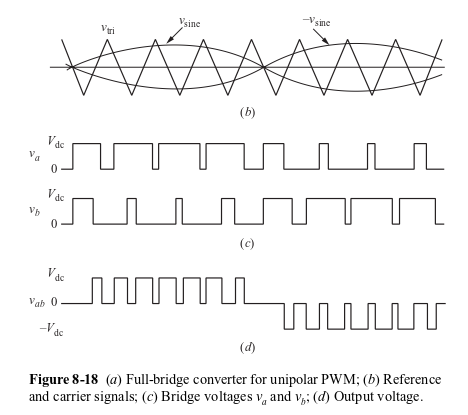
\includegraphics[width=0.7\linewidth]{figs/unipolar_pwm}
		\caption{Funcionamiento del PWM unipolar}
		\label{fig:unipolarpwm}
	\end{figure}
	
	\noindent Además, en el caso de la configuración unipolar se sabe que el valor promedio de $V_{out}$ es aproximadamente igual al promedio de la tensión de control ($V_{ref}$), y su armónico principal se encuentra en $2f_{sw}$. 
	\noindent Un concepto importante el \textit{Índice de Modulación de Amplitud} ($m_a$) el cual se obtiene con la Ec.\eqref{eq:ma}.
	\vspace{0.2 cm}
	\begin{equation}
		m_a = \frac{Vm_{ref}}{Vm_{carrier}}
		\label{eq:ma}
	\end{equation}
	\vspace{0.2 cm}
	De esto se obtiene que si $m_a \leq 1$, entonces la amplitud de la fundamental $V_1$ es  aproximadamente: \[V_1 = 	m_a \cdot V_{dc}\] 
	
	\subsubsection{Análisis de Fourier}
	\noindent Para modelar la carga se busca calcular la carga mediante las siguientes ecuaciones.
	
	\[i_o(t) = \sum_{n=1}^{\infty}I_n \sin(n\omega_o t + \phi_n)\]
	\[I_{rms} = \sqrt{\sum_{n=1}^{\infty} \left(\frac{I_n}{\sqrt{2}}\right)^2}\]
	\[I_n = \frac{V_n}{Z_n} = \frac{V_n}{|R + j\omega L|}\]
	\[P = \sum_{n=1}^{\infty} I_{n,rms}^2	R\]
	
	\section{Diseño}
	\subsection{Margen de tensión}
	El primer cálculo es el margen de tensión que se obtiene de la siguiente manera:
	
	\[m_a = \frac{V_1}{V_{dc}}= \frac{I_{pico} \cdot |Z|}{V_{dc}}\]
	
	\noindent Esto nos permite establecer el índice de modulación que nos solicita cada referencia con la carga dada. Como parte de los diseños $m_a$ no puede llegar a $1$, ya que este valor es fijado por el puente completo y el PR, este último fija $m_{a,max} = 0.92$.\\
	
	Para evitar llegar a este valor límite se busca alcanzar un margen de $80\%$ del $0.92$, por lo tanto:
	
	\[m_a \leq 0.8 \cdot m_{a,max} = 0.736 \]
	
	Ahora se calcula el valor máximo de $|Z|$ de la siguiente forma (tomando $I_{pico} = 1$ A):
	\begin{align*}
		&|Z| \leq \frac{m_a \cdot V_{dc}}{I_{pico}}\\
		&|Z| \leq 13.2\, \Omega
	\end{align*}
	
	\subsection{Rizado de corriente}
	Ahora se calcula el valor del rizado de corriente, el cual determina el valor mínimo de la inductancia:\\
	
	Se sabe que la frecuencia de la señal de salida está a $2f_{sw}$ lo que significa que en el periodo $\frac{T_{sw}}{2}$ se observa un porcentaje de $V_{dc}$. 
	
	\[\Delta t =  D \cdot \frac{T_{sw}}{2}\]
	
	El valor instantáneo de $D$ para este caso corresponde a $D = |m_a \cdot \sin(\omega t)|$ con una frecuencia de $50$ Hz. En el caso de la tensión en el inductor se obtiene mediante lo siguiente:

	\begin{align*}
		&V_L = L \frac{di}{dt}\\
		&\Delta_i = V_L \frac{\Delta_t}{L} \\
		&\Delta_i = \frac{V_{dc} \cdot D(1-D) }{2L\cdot f_{sw}}
	\end{align*}
	
	En el enunciado nos solicitan un rizado máximo de $0.2$ A, por lo que se puede comenzar a calcular los valores del inductor mediante este enunciado.
	
	El peor caso es cuando $D = 0.5$, donde $D(1-D)$ vale $0.25$. En este caso se tiene:
	
	\begin{align*}
		&\Delta_{imax} = \frac{V_{dc}}{8 \cdot L \cdot f_{sw}}\\
		&L \geq \frac{V_{dc}}{8 \cdot \Delta_{imax} \cdot f_{sw}}\\
		&L \geq \frac{18}{8 \cdot 20\text{ kHz} \cdot 0.20 \text{ A}}\\
		&L > 0.56 \text{ mH}
	\end{align*}
	
	Con el fin de evitar el caso máximo de rizado $0.2$ A, $L$ debe ser mayor a $0.56$ mH, por lo que un valor límite adecuado puede ser $0.70$ mH.
	
	\subsection{Potencia}
	 La potencia media en una resistencia depende del valor RMS, no del pico. Para una senoidal:
	 
	 \[I_{rms} = \frac{I_{pico}}{\sqrt{2}}\]
	 \[{I_{rms}}^2 = \frac{{I_{pico}}^2}{2}\]
	 
	 Por lo tanto, si tenemos un valor pico de $1$ A.
	 
	\[{I_{rms}}^2 = 0.5 \text{ A}^2\]
	
	Con este valor se puede calcular el valor de potencia con: 
	
	\[P = {I_{rms}}^2\cdot R = (0.5)\cdot R \]
	
	El enunciado no establece un margen para las resistencias de $5$ W por lo que se establecerá un margen del 50\%.
	
	\[\frac{0.5 \cdot R }{N} \leq 2.5\text{ W}\]
	\[R \leq 5N\, \Omega\]

	Con dos resistencias el límite es $10\ \Omega$ y con tres es $15\ \Omega$. En este cálculo $R$ es la resistencia externa, porque es la que disipan las resistencias.

	\subsection{Tiempo muerto}
	Durante el tiempo muerto los dos MOSFET de una pierna están apagados y la tensión de salida depende del signo de la corriente. Cada pierna pierde en promedio $t_d \cdot f_{sw} \cdot V_{dc}$, y las dos piernas se suman en la tensión de la carga. Con $t_d = 1\ \mu$s:

	\[V_e = 2 \cdot t_d \cdot f_{sw} \cdot V_{dc} = 0.72 \text{ V}\]

	Este valor es una cota, porque el tiempo muerto efectivo se reduce por los retardos de las compuertas. El error tiene forma de onda cuadrada en fase con la corriente, por lo que su fundamental es:

	\[V_{e,1} = \frac{4 \cdot V_e}{\pi} = 0.92 \text{ V}\]

	El caso más difícil es la referencia de $0.2$ A pico, porque es la que pide menos tensión. Se propone que el error no supere el $50\%$ de esa tensión ($a = 0.5$), lo que da la resistencia mínima:

	\begin{align*}
		&V_{e,1} \leq a \cdot I_{min} \cdot R\\
		&R \geq \frac{V_{e,1}}{a \cdot I_{min}} = \frac{0.92 \text{ V}}{0.5 \cdot 0.2 \text{ A}}\\
		&R \geq 9.2\, \Omega
	\end{align*}

	Aquí $R$ es la resistencia total de la carga, incluidos el devanado, el shunt y los dos MOSFET en conducción.

	\subsection{Corriente del inductor}
	Con el controlador saturado en $m_{a,max}$ la corriente queda limitada por la resistencia total. El inductor debe soportar esa corriente sin saturarse.

	\[I_{max} = \frac{m_{a,max} \cdot V_{dc}}{R}\]

	Con $R = 9.2\ \Omega$ se obtiene $I_{max} = 1.8$ A, y con $R = 10\ \Omega$ se obtiene $I_{max} = 1.7$ A.

	\subsection{Ventana de diseño}
	Al juntar los límites anteriores, con $V_{dc} = 18$ V y $f_{sw} = 20$ kHz, la carga debe cumplir con lo siguiente:
	\vspace{0.3 cm}
	\begin{itemize}
		\item Resistencia total, $9.2\ \Omega \leq R \leq 13.2\ \Omega$
		\item Resistencia externa con dos resistencias de $5$ W, $R_{ext} \leq 10\ \Omega$
		\item Inductancia, $L \geq 0.70$ mH
		\item Corriente del inductor, al menos $1.7$ A con $R = 10\ \Omega$
	\end{itemize}

	\subsection{Punto de diseño candidato}
	Se toma como candidato $R = 10\ \Omega$ y $L = 2$ mH. La resistencia externa se forma con dos resistencias de $4.7\ \Omega$ y $5$ W en serie, $R_{ext} = 9.4\ \Omega$, y el resto de $R$ corresponde al devanado, al shunt y a los MOSFET. Estos valores deben confirmarse con la carga medida.

	\[\omega L = 2\pi \cdot 50 \text{ Hz} \cdot 2 \text{ mH} = 0.63\ \Omega\]
	\[|Z| = |10 + j0.63|\ \Omega = 10.02\ \Omega\]

	El Cuadro \ref{tab:candidato} resume los tres puntos de operación, donde $P_{ext}$ es la potencia en las dos resistencias externas.

	\begin{table}[H]
		\centering
		\caption{Puntos de operación con $R = 10\ \Omega$, $L = 2$ mH y $V_{dc} = 18$ V}
		\label{tab:candidato}
		\begin{tabular}{ccccc}
			\hline
			$I_{pico}$ (A) & $V_1$ (V) & $m_a$ & $\Delta_{imax}$ (A) & $P_{ext}$ (W) \\
			\hline
			$0.2$ & $2.00$ & $0.111$ & $0.022$ & $0.19$ \\
			$0.5$ & $5.01$ & $0.278$ & $0.045$ & $1.18$ \\
			$1.0$ & $10.02$ & $0.557$ & $0.056$ & $4.70$ \\
			\hline
		\end{tabular}
	\end{table}

	En los tres puntos $m_a$ queda bajo $0.736$ y el rizado bajo $0.20$ A. A $1$ A pico el rizado se calcula con $D = 0.5$, porque el índice pasa por ese valor durante el ciclo. Cada resistencia de $4.7\ \Omega$ disipa $2.35$ W, un $47\%$ de su potencia nominal.

	\subsection{Ensayo de cambio de resistencia}
	El enunciado pide un cambio de al menos $25\%$ sobre la resistencia externa, con $0.5$ A pico. Con una resistencia adicional de $2.7\ \Omega$ en serie:

	\[R_{ext} = 9.4\ \Omega + 2.7\ \Omega = 12.1\ \Omega\]
	\[\frac{12.1 - 9.4}{9.4} = 28.7\%\]

	La resistencia total sube a $R = 12.7\ \Omega$, con lo que se obtiene:

	\begin{align*}
		&|Z| = |12.7 + j0.63|\ \Omega = 12.72\ \Omega\\
		&V_1 = 0.5 \text{ A} \cdot 12.72\ \Omega = 6.36 \text{ V}\\
		&m_a = \frac{6.36 \text{ V}}{18 \text{ V}} = 0.353\\
		&P_{ext} = \frac{(0.5 \text{ A})^2}{2} \cdot 12.1\ \Omega = 1.51 \text{ W}
	\end{align*}

	Los dos puntos del ensayo quedan dentro de los límites de tensión y de disipación.
	\section{Sensor de Corriente}
	Para esta sección se plantea el uso de un Sensor de corriente basado en efecto de Hall, ACS712. Este sensor permite medir la corriente de forma directa a diferencia de los sensores de efecto de Hall convencionales. Este sensor permite la medición bi-dirección, adecuado para esta aplicación ya que se trabaja con una corriente AC. Además, este modelo cuenta aislamiento entre sus terminales de entrada por lo que simplifica las etapas a diseñar para este módulo.
	
	\subsection{Características del ACS712 - Consideraciones de Interés}
	\begin{figure}[H]
		\centering
		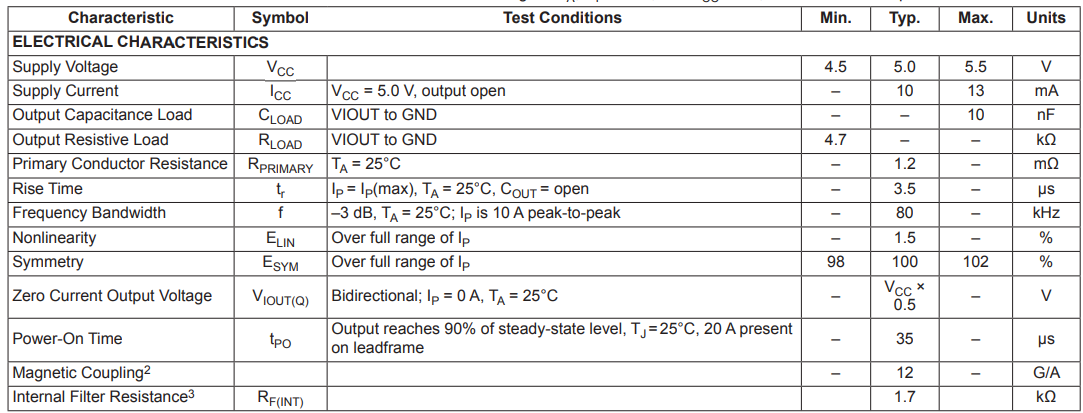
\includegraphics[width=0.8\linewidth]{figs/caracteristicas_sensor_de_Corriente}
		\caption{Caracteristicas Electricas}
		\label{fig:caracteristicassensordecorriente}
	\end{figure}
	
	Debido a las características de este sensor se deberá implementar una fuente de tensión adicional de $5$ V, ya que no se podrá alimentar por la FPGA. Esto se debe a que las salidas de la Basys 3 son de $3.3$ V y el sensor necesita los $5$ V. Otro inconveniente del sensor es su voltaje de salida, ya que si la corriente es de $0$ A, la tensión de salida es $V_{cc}/2$, lo cual tendrá que ser adecuado para conectarse al JXADC, debido a que supera el umbral de los $1.8$ V para indicar el estado.
	
	 
	\subsubsection{Circuito de Referencia}
	
	
	\begin{figure}[H]
		\centering
		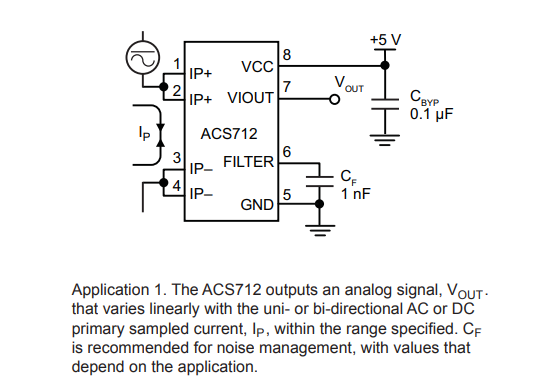
\includegraphics[width=0.6\linewidth]{figs/circuito_medidor_de_corriente}
		\caption{Circuito de medición de corriente}
		\label{fig:circuitomedidordecorriente}
	\end{figure}
	
	
	
	
	
	
	
	
\end{document}
